\documentclass{oblivoir}
\usepackage{graphicx}
\usepackage{fapapersize}
\usefapapersize{*,*,30mm,*,30mm,*}

\usepackage{amsmath}
\usepackage{amsthm}
\theoremstyle{definition}
\newtheorem{exercise}{연습문제}
\newtheorem{homework}[exercise]{숙제}
\newtheorem{example}[exercise]{예제}

\usepackage{color}

\usepackage{url}

\usepackage{tikz}

\newcommand{\inv}[1]{\textcolor{blue}{\ensuremath{[{#1}]}}}

\begin{document}
\title{Potpourri}
\author{강지훈 (\url{http://sf.snu.ac.kr/jeehoon.kang})}
\maketitle

\begin{abstract}
  여러가지 예제를 통해 문제해결기법, 즉 알고리즘을 고안하는 법을
  연습한다.  널리 알려진 이분 검색 문제에서부터 출발하여, KAIST
  문제해결기법 강좌에서도 예제로 쓰이는 연속된 숫자들의 합 문제를
  살펴보고 그 문제를 어떻게 변형할 수 있는지 살펴본다. 그리고 Fiver
  Game 문제를 소개하고 이 문제를 어떻게 풀 수 있을지 생각해본다.
  마지막으로 문제해결기법과 관한 저자의 경험을 소개하며 마친다.
\end{abstract}

\begin{exercise}
Potpourri가 뭘까?
\end{exercise}

\section{이분 검색}
오름차순\footnote{보다 정확히는, 비내림차순}으로 정렬된 배열 $A$에서 값
$v$가 있는지, 있다면 몇번째 원소인지 찾아보자.

\paragraph{간단한 방법}
가장 간단한 방법은 배열에 있는 원소를 하나씩 살펴보는 것이다:
\begin{align*}
\texttt{10:}& \texttt{find(v: int, A: int[N]): bool :=} \\
\texttt{11:}& \ \ \texttt{for (i := 0; i < N; ++i) \{} \\
\texttt{12:}& \ \ \ \ \texttt{if (v = A[i]) return i} \\
\texttt{14:}& \ \ \texttt{\}} \\
\texttt{15:}& \ \ \texttt{return -1}
\end{align*}
\noindent 그러나 이 방법은 $N$개의 원소를 모두 확인해야하기 때문에
시간이 오래 걸린다.\footnote{보다 ``고상한'' 표현으로는, $O(N)$의
  시간복잡도를 가진다.}  이보다 더 좋은 방법은 없을까?  만약 배열이
오름차순으로 정렬되어있지 않다면, 배열의 원소를 하나하나 뒤져보는
수밖에 없을 것이다. 

\paragraph{더 나은 방법}
배열이 정렬되어있을 경우에도 그럴까?
\begin{exercise}[이분 검색]
  더 빠른 알고리즘을 고안하라.  아래 모범 답안을 보기 전에 충분히
  생각해보자.
  \begin{align*}
    \texttt{10:}& \texttt{find(v: int, A: int[N]): bool :=} \\
    \texttt{11:}& \ \ \texttt{l := -1, r := N} \\
    \texttt{12:}& \ \ \texttt{while (l + 1 < r) \{} \\
    \texttt{13:}& \ \ \ \ \texttt{m := (l + r) / 2} \\
    \texttt{14:}& \ \ \ \ \texttt{if (A[m] < v) l := m} \\
    \texttt{16:}& \ \ \ \ \texttt{else r := m} \\
    \texttt{19:}& \ \ \texttt{\}} \\
    \texttt{20:}& \ \ \texttt{return (A[r] = v) ? r : -1}
  \end{align*}
\end{exercise}

어떻게 $N$개의 원소를 다 확인해보지 않고도 위 알고리즘이 옳을 수
있을까?  ``왜'' 그런지 잠깐 생각해보자.

\begin{exercise}[이분 검색이 옳음]
  위 알고리즘은 왜 옳을까? 힌트: 변수의 의미는 \texttt{l}eft,
  \texttt{r}ight, \texttt{m}iddle이며, left, right는 우리가 관심있는
  범위를 나타낸다.  위 알고리즘은 가운데(middle) 있는 원소와 $v$를
  비교한 뒤 (line 14, $(A[m] < v)$), 범위를 줄여나간다.
\end{exercise}

\paragraph{알고리즘 고안하는 방법}
이분 검색을 살펴보며 확인했듯, 알고리즘을 고안할 때에는 일반적으로 다음
과정을 거쳐야 한다:
\begin{itemize}
\item 가장 자명한 답을 고안한다.
\item 이 답이 충분히 훌륭하다면 그만 멈춘다.
\item 그렇지 않다면, 지금 생각한 답이 고려하지 않은 성질이 있는지
  확인한다.  문제의 성질일 수도 있고, 주어지는 입력의 성질일 수도
  있다.
\item 그 성질을 이용해서 알고리즘을 더 좋게 만들 수 있을지 생각해본다.
\item 충분히 좋은 알고리즘을 얻을 때까지 반복한다.
\end{itemize}

\paragraph{} 숙제와 알고리즘의 핵심을 찌르는 질문 하나 보고 나가자.

\begin{homework}
  이분 검색 알고리즘을 구현하라.  참고로, 앞으로 모든 숙제의 입력/출력
  파일 형식 및 예제는 조교가 앞으로 공지할 예정이다.
\end{homework}

\begin{exercise}[이분 검색의 이름]
  왜 이 알고리즘의 이름은 ``이분 검색''일까?
\end{exercise}

\section{연속된 숫자들의 합}

다음과 같은 배열이 있다고 하자:
\[
A: \begin{array}{|c|c|c|c|c|c|c|c|c|c|}
\hline
1 & -3 & 5 & 4 & -19 & 23 & -3 & 0 & 4 & -2 \\
\hline
\end{array}
\]
이중 연속된 숫자들을 골라 합을 구해보자.  예컨데 $1+(-3)+5=3$,
$(-19)+23+(-3)+0=1$.  이런 합중에서 가장 큰 숫자를 찾아보자.

\paragraph{간단한 방법}
가장 간단한 방법은 모든 합을 다 고려해보는 것이다. 합은 약 $N^2$개
있고, 합을 구할 때는 약 $N$개의 숫자를 더해야 하므로, 대략 $N^3$에
비례하는 시간이 걸린다.\footnote{고상하게는, $\Theta(N^3)$의
  시간복잡도를 가진다.}

\paragraph{더 나은 방법}
더 나은 방법은 없을까?  이 문제는 연속된 숫자의 합에 관심이 있으므로,
연속된 숫자들을 더해보자.  아래에서 모든 $i$에 대해,
$S[i] = A[0] + A[1] + \cdots + A[i]$이다:
\[
S: \begin{array}{|c|c|c|c|c|c|c|c|c|c|}
\hline
1 & -2 & 3 & 7 & -12 & 11 &  8 & 8 & 12 & 10 \\
\hline
\end{array}
\]
\begin{exercise}
  $S$를 이용해서, 즉 우리가 연속된 숫자의 합에 관심이 있다는 성질을
  이용해서 더 좋은 알고리즘을 고안하라.

  고안한 알고리즘이 정말 최선일까?  더 좋은 알고리즘이 있을까?
\end{exercise}

핵심을 찌르는 질문 하나 보고 가자.

\begin{exercise}[왜 이 문제를?]
  우리는 왜 하필이면 이 문제를 공부했을까?
\end{exercise}

\subsection{변형 문제: 2차원}

다음과 같은 배열이 있다고 하자:
\[
A: \begin{array}{|c|c|c|c|c|c|c|c|c|c|}
\hline
1 & -3 & 5 & 4 & -19 & 23 & -3 & 0 & 4 & -2 \\
\hline
7 & 4 & -13 & 8 & -3 & 3 & 3 & 13 & -4 & -10 \\
\hline
-30 & -3 & 3 & 4 & 13 & -29 & 3 & -1 & -1 & -2 \\
\hline
\end{array}
\]
이중 직사각형을 골라 합을 구해보자.  예컨데 $[1+(-3)+5] + [7+4+(-13)]=1$,
$[23+(-3)]+[3+3]+[(-29)+3]=0$.  이런 합중에서 가장 큰 숫자를 찾아보자.

\begin{exercise}
  가장 간단한 방법은 무엇일까?
\end{exercise}

\begin{exercise}
  원래 문제에서 $S$를 이용한 것 같이 이 문제에서도 뭔가 이용할만한게
  있을까?
\end{exercise}

\begin{homework}
  간단한 방법보다 더 좋은 알고리즘을 고안하라.
\end{homework}

\begin{exercise}
  3차원 문제로 확장할 수 있을까? $N$차원 문제로 확장할 수 있을까?
\end{exercise}

\section{Fiver Game}
동전을 원형으로 $N$개 늘여놓아보자.  동전은 앞면(H)이 위로 놓여져
있거나, 뒷면(T)이 위로 놓여져 있다.  예를들어 다음은 5개의 동전을
늘여놓은 모습이다:
\begin{center}
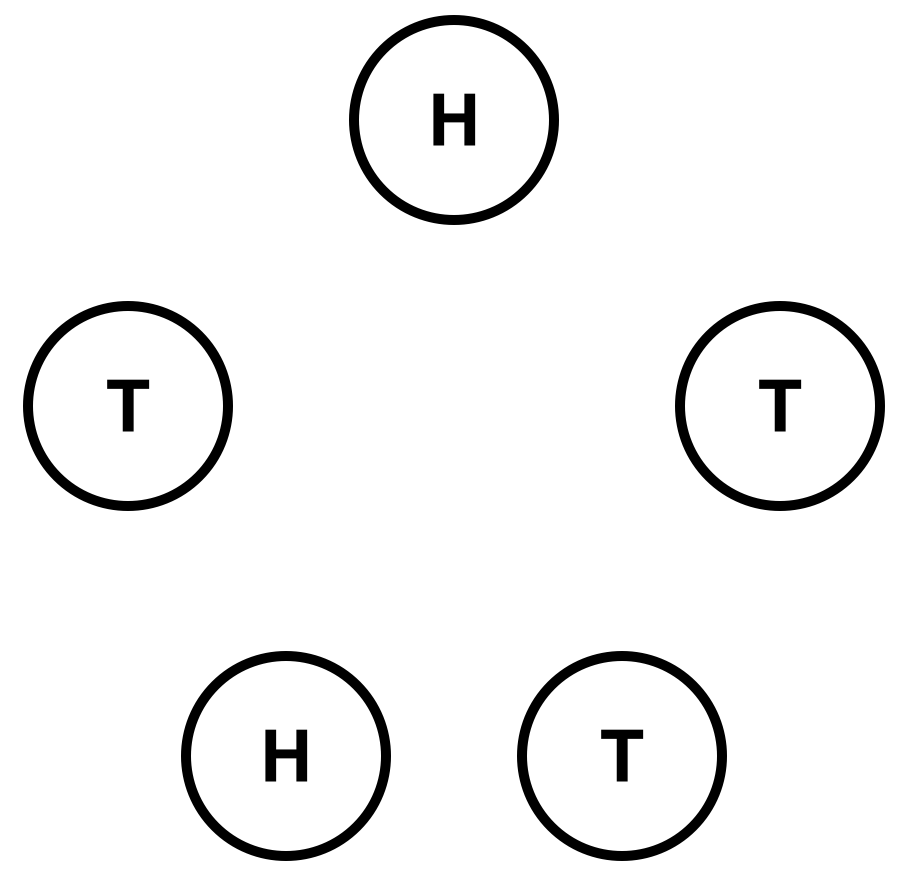
\includegraphics[width=100px]{p1.png}
\end{center}
우리는 이중 연속된 $M$개의 동전을 한꺼번에 뒤집을 수 있다.  예를들어
$M=3$인 경우 아래 3개의 동전을 뒤집을 수 있다:
\begin{center}
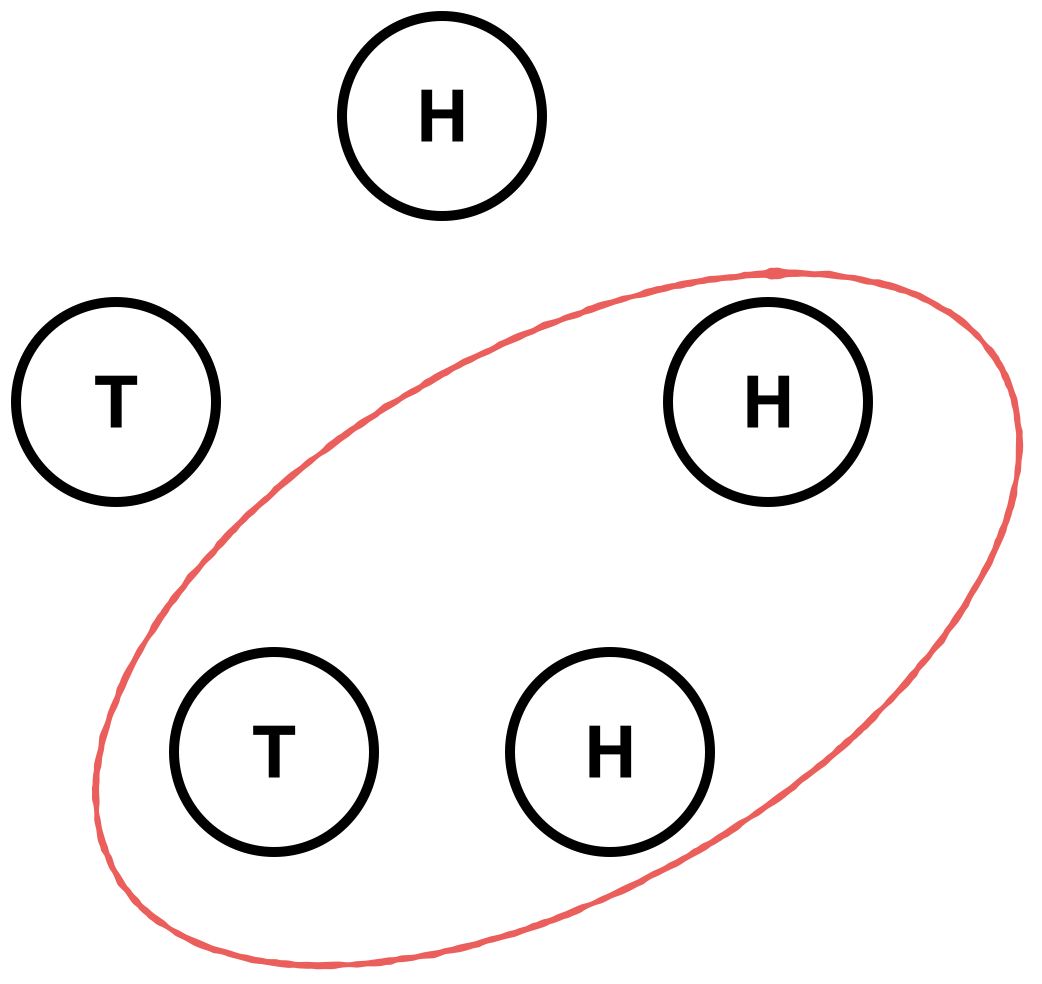
\includegraphics[width=100px]{p2.png}
\end{center}

동전을 계속 뒤집어서 모든 동전이 앞면이 되도록 만들 수 있을까?

\begin{homework}
  위 문제를 푸는 프로그램을 작성하라.
  \begin{itemize}
  \item 입력: $N$과 $M$이 주어지고, 동전의 정보가 $N$개 주어진다. 각
    정보는 H거나 T이다.
  \item 출력: Yes 혹은 No.
  \end{itemize}
\end{homework}

\begin{exercise}
  문제를 풀기 전에, 잠시 실제 동전을 가지고 Fiver Game을 즐겨보자!
\end{exercise}

문제를 풀 때, 위에서 언급한 ``알고리즘 고안하는 방법''을 참조하라.

\begin{exercise}
  2차원 문제로 확장할 수 있을까? $N$차원 문제로 확장할 수 있을까?  동전
  대신 $K$면 주사위를 쓰면 어떻게 될까?  다음 논문을 참고하라:
  \cite{DBLP:journals/combinatorics/KangKP12}
\end{exercise}

\section{마치며}
문제해결기법을 공부하는 학생들에게 항상 해주는 이야기가 있다.  2003년
KOI 중등부 1번 문제는 그래프의 최단거리를 구하는 문제였다.  나는 아는
문제가 나와서 기뻐하며 다음과 같이 Floyd-Warshall 알고리즘을 작성했다:
\begin{align*}
& \texttt{for \texttt{i} := 1 to n do} \\
& \ \ \texttt{for \texttt{j} := 1 to n do} \\
& \ \ \ \ \texttt{for \texttt{k} := 1 to n do} \\
& \ \ \ \ \ \ \texttt{if (d[i][k] > d[i][j] + d[j][k])} \\
& \ \ \ \ \ \ \ \ \texttt{d[i][k] := d[i][j] + d[j][k]}
\end{align*}
하지만 위 알고리즘은 \emph{틀렸다}.  올바른 알고리즘은, 루프를
\emph{\texttt{k}부터} 돌려야 한다:
\begin{align*}
& \texttt{for \texttt{k} := 1 to n do} \\
& \ \ \texttt{for \texttt{i} := 1 to n do} \\
& \ \ \ \ \texttt{for \texttt{j} := 1 to n do} \\
& \ \ \ \ \ \ \texttt{if (d[i][k] > d[i][j] + d[j][k])} \\
& \ \ \ \ \ \ \ \ \texttt{d[i][k] := d[i][j] + d[j][k]}
\end{align*}
내가 이 문제를 틀렸던 까닭은, 알고리즘이 왜 맞는지에 대한 이해 없이,
무조건 알고리즘을 외워서 대회에서 써먹으려고 했기 때문이다.  알고리즘이
왜 맞는지 깊게 고민해봐야만, 대회에서 문제를 만났을 때 자신 있게
알고리즘을 적용할 수 있다.  이는 쉬운 문제나 어려운 문제, 그리고
궁극적으로 현업에서 만날 문제에 이르기까지 변치 않는 중요한 원칙이다.
여러분들은 알고리즘이 왜 옳은지 깊게 고민해서, 내가 대회에서 저질렀던
어이없는 실수를 저지르지 않길 바란다.

\begin{homework}
  Floyd-Warshall 알고리즘은 왜 옳을까?  간단한 에세이를 써서 제출하라.
  힌트: $\texttt{k}$는 경로가 방문하는 노드의 수와 관련이 있다.
\end{homework}

참고로 이 문서는 GitHub로 관리되고 있다:
\url{https://github.com/jeehoonkang/doc-invariant}

\bibliographystyle{abbrv}
\bibliography{references}

\end{document}
